% Author: Vitaly Parnas
\documentclass{article}

\usepackage{tikz}
% \usepackage[legalpaper, landscape, margin=2in]{geometry}
\usepackage[paperheight=13in,paperwidth=13in,margin=1in,heightrounded]{geometry}
\usepackage{amsmath}
\usetikzlibrary{mindmap,trees}
\usepackage{verbatim}
\graphicspath{ {images/} }

\begin{document}
\pagestyle{empty}

\begin{comment}
:Title: Parallel Processing Mind Map
:Tags: Manual, Mindmap

| Author: Vitaly Parnas
| Source: UIC Parallel Processing course material

\end{comment}

\begin{tikzpicture}[mindmap, grow cyclic, every node/.style=concept,
    concept color=black,text=white,
    level 1/.append style={font=\Large\bfseries,level distance=8cm,sibling angle=90},
    level 2/.append style={font=\small\bfseries,level distance=4cm,sibling angle=45},
    level 3/.append style ={font=\tiny\bfseries},
    nucleus/.style= {concept, font=\huge\bfseries},
    ]

    % mbox content remains on one line
    \node [nucleus] {Parallel \mbox{Processing}\\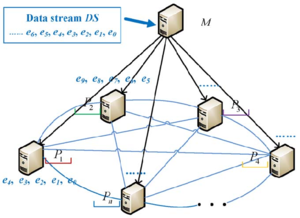
\includegraphics[width=3.5cm,height=3.5cm,keepaspectratio]{nucleus}}
    child[concept color=green!50!white,text=black] { node {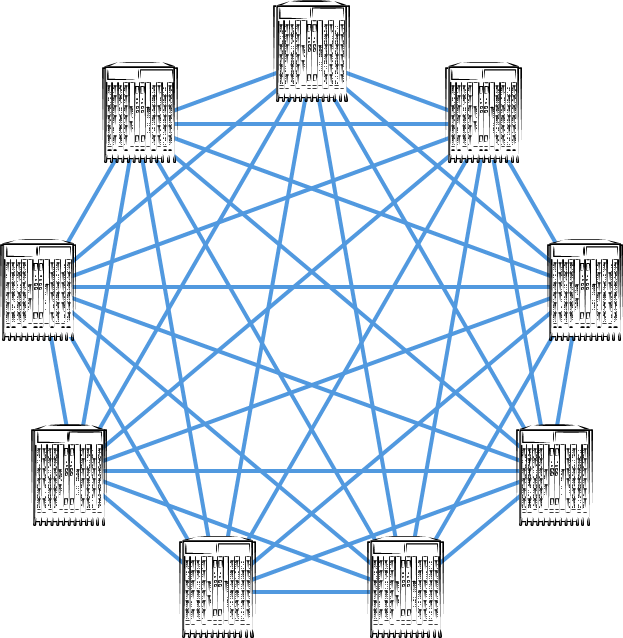
\includegraphics[width=2cm,height=2cm,keepaspectratio]{topology}\\Models}
        child { node {Linear Array} }
        child { node {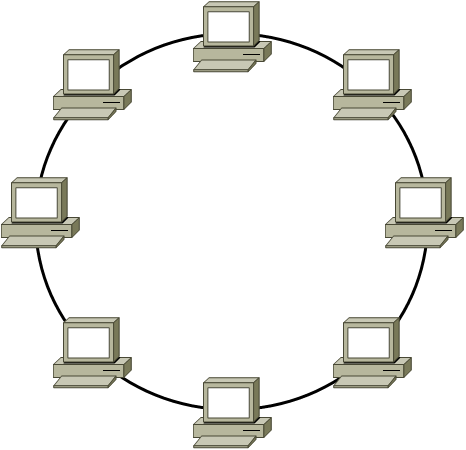
\includegraphics[width=2cm,height=2cm,keepaspectratio]{ring_topology}\\Ring} }
        child { node {
\includegraphics[width=2cm,height=2cm,keepaspectratio]{mesh}\\Mesh} }
        child { node {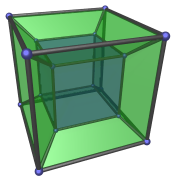
\includegraphics[width=2cm,height=2cm,keepaspectratio]{hypercube_2}\\Hypercube} }
        child { node {K\-ary d\-cube\\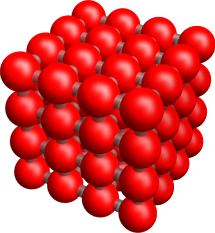
\includegraphics[width=2cm,height=2cm,keepaspectratio]{kary_dcube}} }
        child { node {Binary tree} }
        child { node {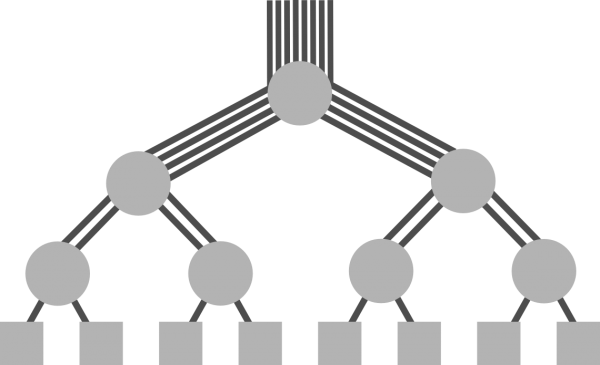
\includegraphics[width=2cm,height=2cm,keepaspectratio]{fat_tree}\\Fat Tree} }
    }
    child[concept color=blue!50!white,text=black] { node {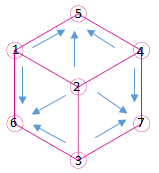
\includegraphics[width=2cm,height=2cm,keepaspectratio]{hypercube_comm}\\Communication}
        child { node {One-to-all Broadcast} }
        child { node {All-to-all Broadcast} }
        child { node {Scatter} }
        child { node {Gather} }
        child { node {Reduce} }
        child { node {All-to-all Personal} }
        child { node {Prefix Sum} }
        child { node {Cartesian Shift} }
    }
    child[concept color=red!50!white,text=black] { node {Performance/\\Scalability\\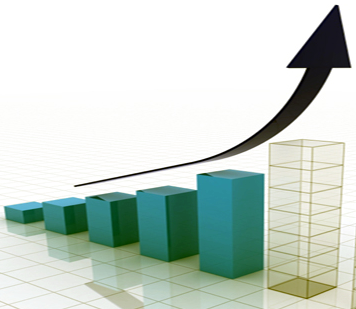
\includegraphics[width=2cm,height=2cm,keepaspectratio]{performance}}
        child { node {Serial Runtime $T_s$} }
        child { node {Parallel Runtime $T_p$} }
        child { node {Speedup $S = T_s/T_p$} }
        child { node {Overhead $T_o = pT_p - T_s$} }
        child { node {Efficiency $E = S/p$} }
        child { node {ISO func} }
    }
    child[concept color=orange!50!white,text=black] { node {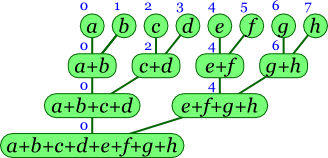
\includegraphics[width=3cm,height=3cm,keepaspectratio]{parallel_alg}\\Algorithms}
        child{ node {Matrix} 
            child[sibling angle=90] { node {Multiplication} 
                child { node {Traditional}}
                child { node {Canon}}
                child { node {Strassen}}
            }
            child { node {LU Decomposition} 
                child { node {Block 1D part}}
                child { node {Block 2D part}}
                child { node {Pipeline}}
                child { node {Sequential part}}
                child { node {Cyclic part}}
            }
        }
        child { node {Sorting} 
            child { node {Bitonic} }
            child { node {Bubble} }
            child { node {Quicksort} }
        }
        child { node {Graph} 
            child { node {Prim's MST} }
            child { node {Single Source Shortest Path} }
            child { node {All Pairs Shortest Path} 
                child { node {Source Part} }
                child { node {Hypercube} }
                child { node {Mesh} }
            }
        }
        child { node {Discreete Optimization} }
    }
    ;
\end{tikzpicture}\end{document}
